\documentclass[12pt]{article}
\usepackage{graphicx}
\usepackage[colorlinks=true, urlcolor=black]{hyperref}
\title{Sistema Acad\'emico Fractal\\Manual del Docente}
%\author{Edson A. Ticona Zegarra}
\date{Abril 2019}

\renewcommand{\figurename}{Figura}
\begin{document}
\maketitle

\section{Login}
Al ingresar a la direcci\'on \url{www.fractal.edu.pe:9000/asistencias/} 
\footnote{Todas las im\'agenes contienen otra direcci\'on (URL) que no debe ser tomada en cuenta.}
se muestra la p\'agina de la figura~\ref{fig:login}.
Ingresar con su usuario y contrase\~na. Las credenciales de acceso son estrictamente de uso personal y
se recomienda extremo cuidado en no usar contrase\~nas simples.
\begin{figure}[ht]
  \centering
  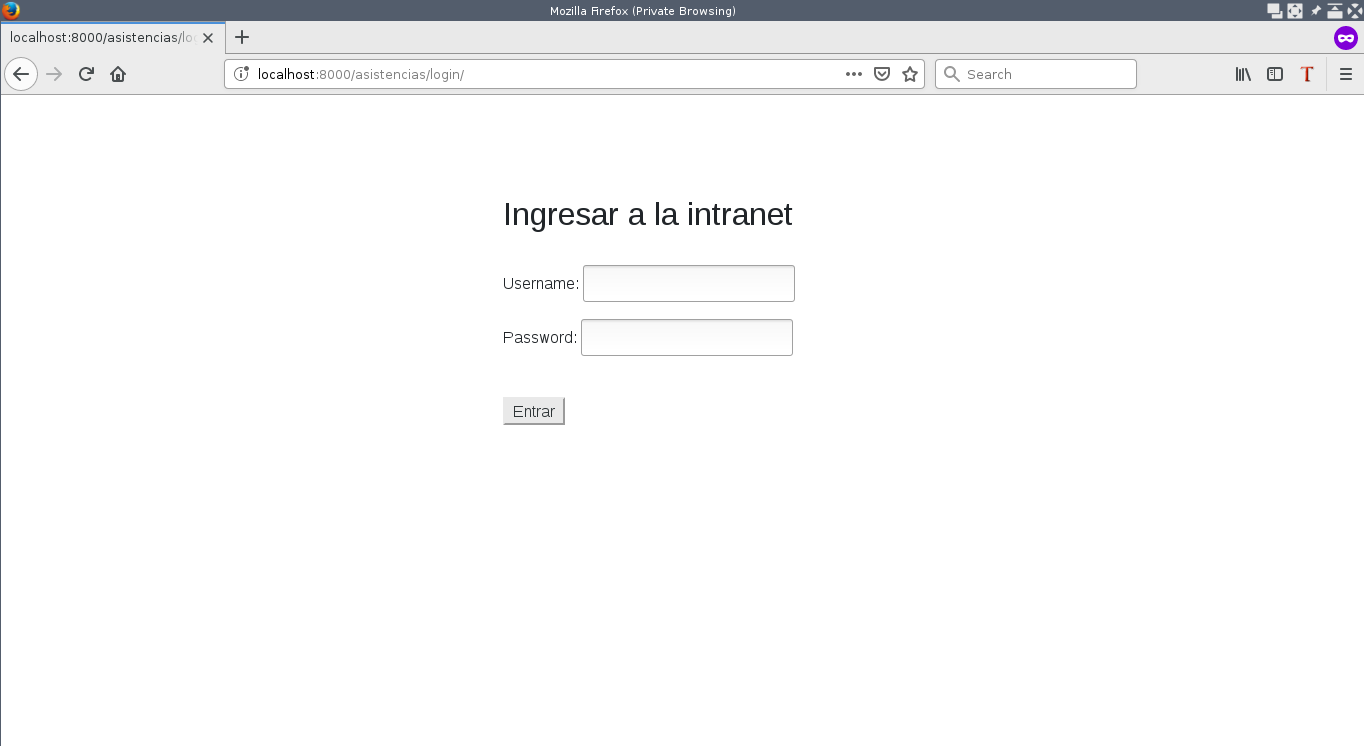
\includegraphics[width=0.8\textwidth]{images/login.png}
  \caption{P\'agina de login}
  \label{fig:login}
\end{figure}

\section{Notas Diarias}
Una vez logeado, la primera p\'agina en mostrarse al usuario es aquella que permite ingresar las notas
diarias de los estudiantes. En la parte superior se puede ver la barra de navegaci\'on con los dos menus
disponibles al lado izquierdo; al lado derecho, se muestra el nombre del docente (``profesor test``) y
la opci\'on de Salir.

Debajo de la barra de navegaci\'on se ve el grado y secci\'on asignados al docente. A continuaci\'on se
muestra la fecha a la que corresponde la evaluaci\'on; que por defecto se considera el d\'ia actual. 
Luego, seleccionar un curso y aparecer\'a la lista de estudiantes que corresponde al grado y secci\'on
\begin{figure}[ht]
  \centering
  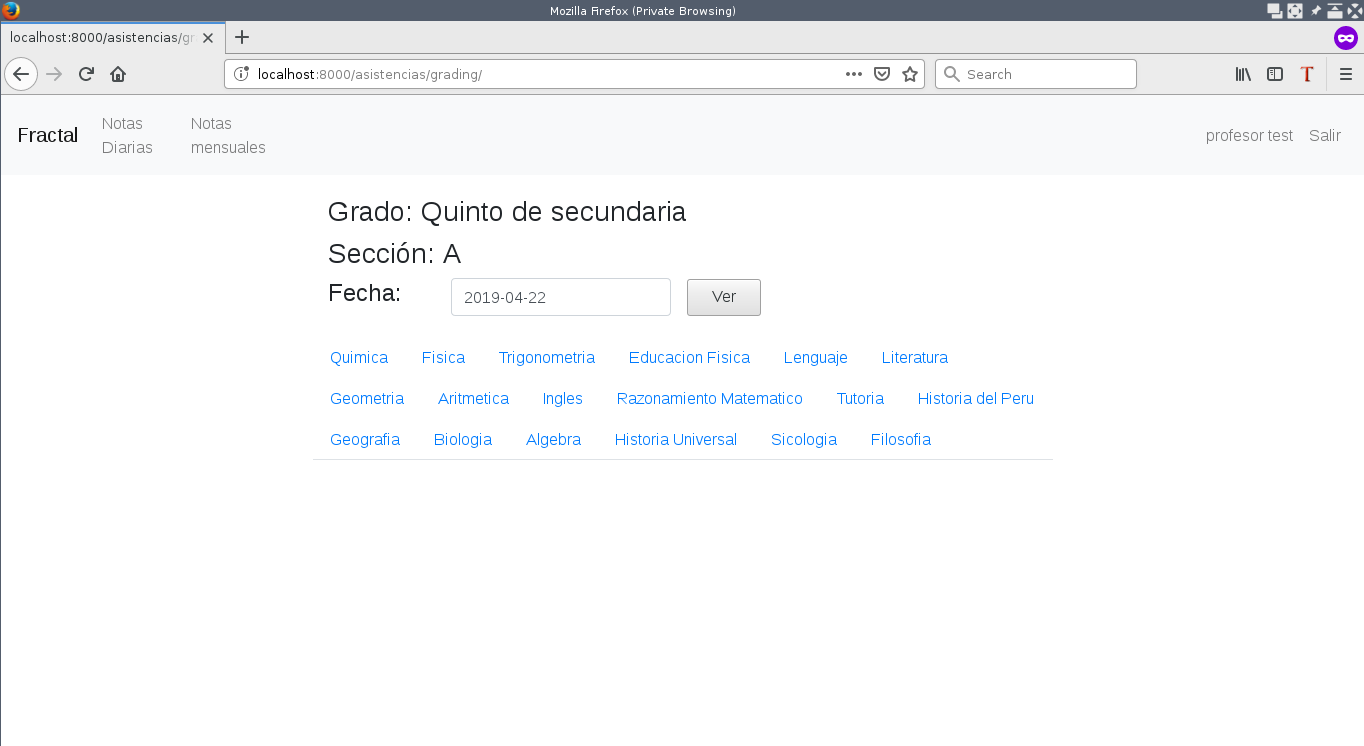
\includegraphics[width=0.8\textwidth]{images/profesor1.png}
  \caption{Registro diario de notas}
  \label{fig:profesor1}
\end{figure}

Ingresar las notas del curso seleccionado y hacer click en el boton guardar que esta en la parte
inferior de la p\'agina, como se ve en la figura~\ref{fig:profesor6}.
\textbf{Las notas guardadas son solo del curso que se muestra, si se modific\'o
notas de otros cursos, el boton guardar solo guardar\'a las notas del curso en pantalla}
\begin{figure}[ht]
  \centering
  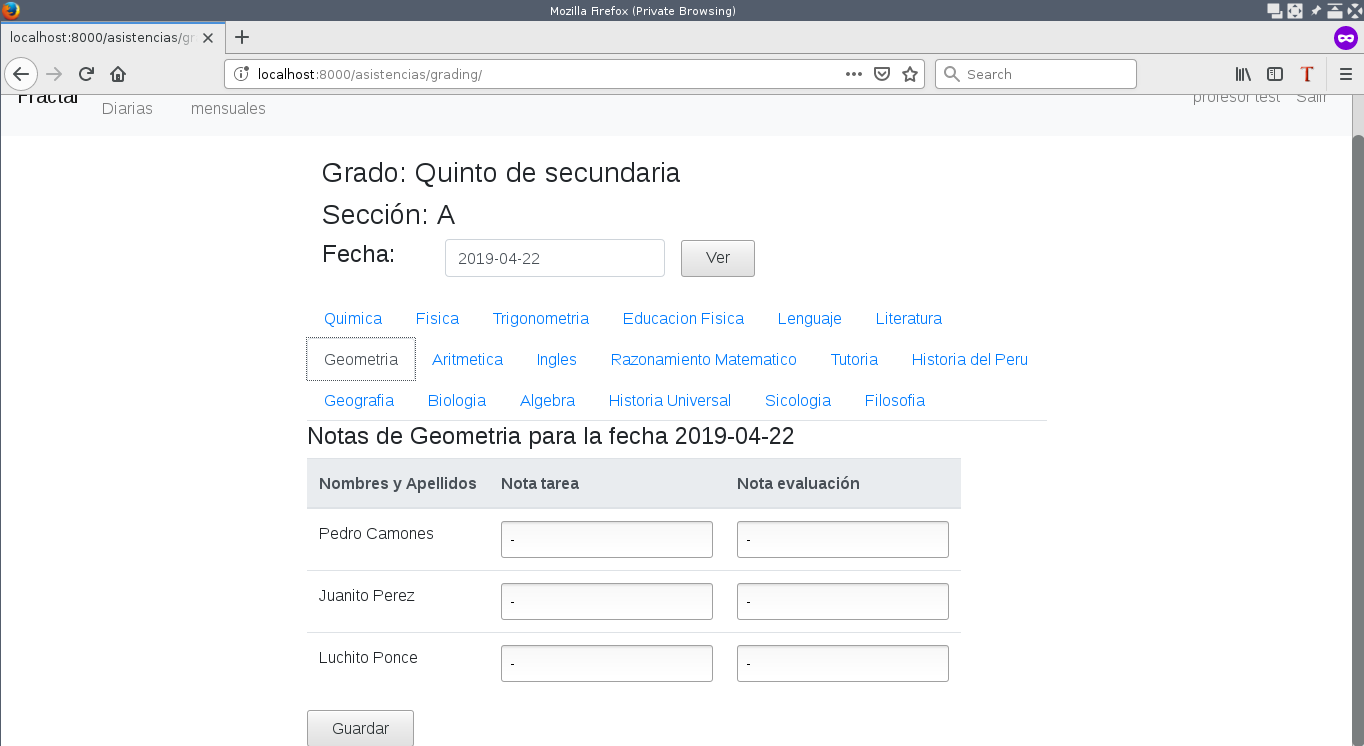
\includegraphics[width=0.8\textwidth]{images/profesor6.png}
  \caption{Registro diario de notas}
  \label{fig:profesor6}
\end{figure}

\newpage
Si se desea ingresar las notas de otro d\'ia, al hacer click en la fecha se abrir\'a un calendario
como se muestra en la imagen~\ref{fig:profesor2}.
\begin{figure}[ht]
  \centering
  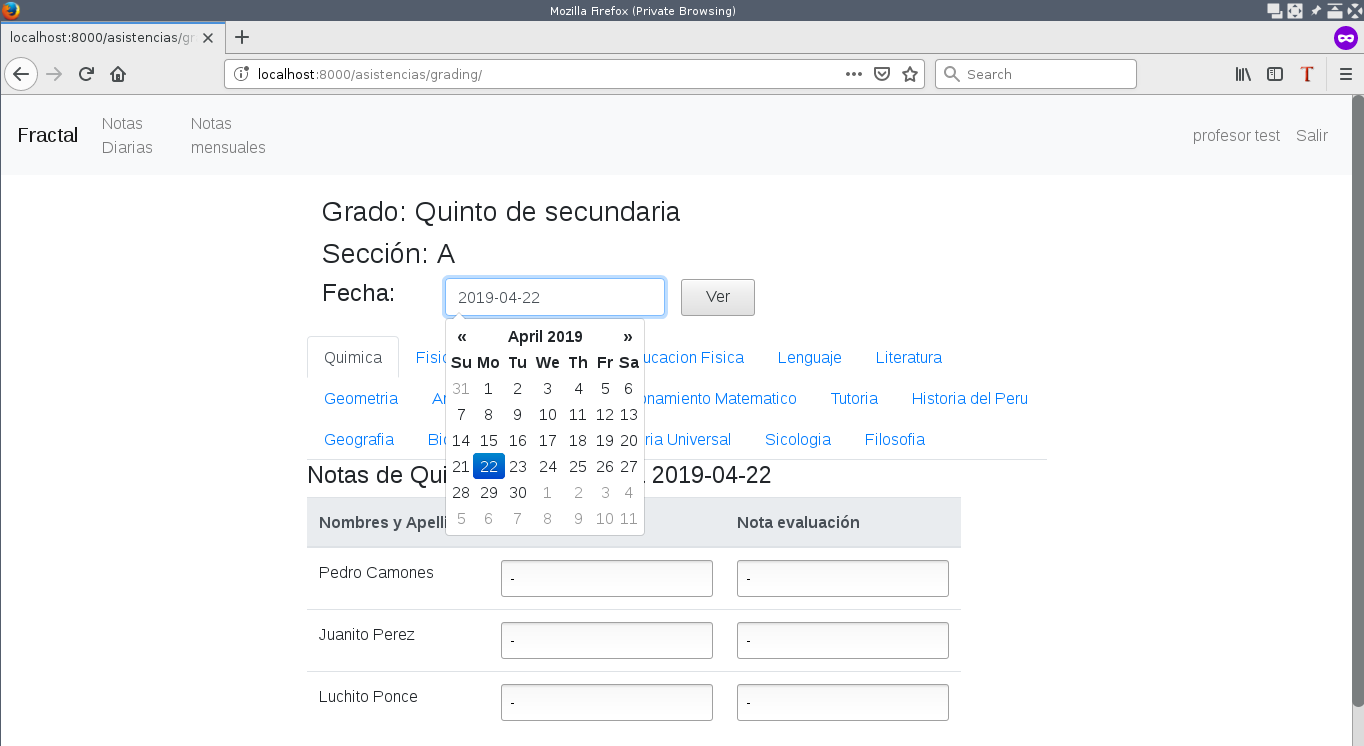
\includegraphics[width=0.8\textwidth]{images/profesor2.png}
  \caption{Registro diario de notas}
  \label{fig:profesor2}
\end{figure}

En caso de seleccionar una fecha no v\'alida, como domingos, vacaciones  feriados, se muestra un
mensaje de fondo amarillo indicando que no es posible ingresar notas para esa fecha.
\begin{figure}[ht]
  \centering
  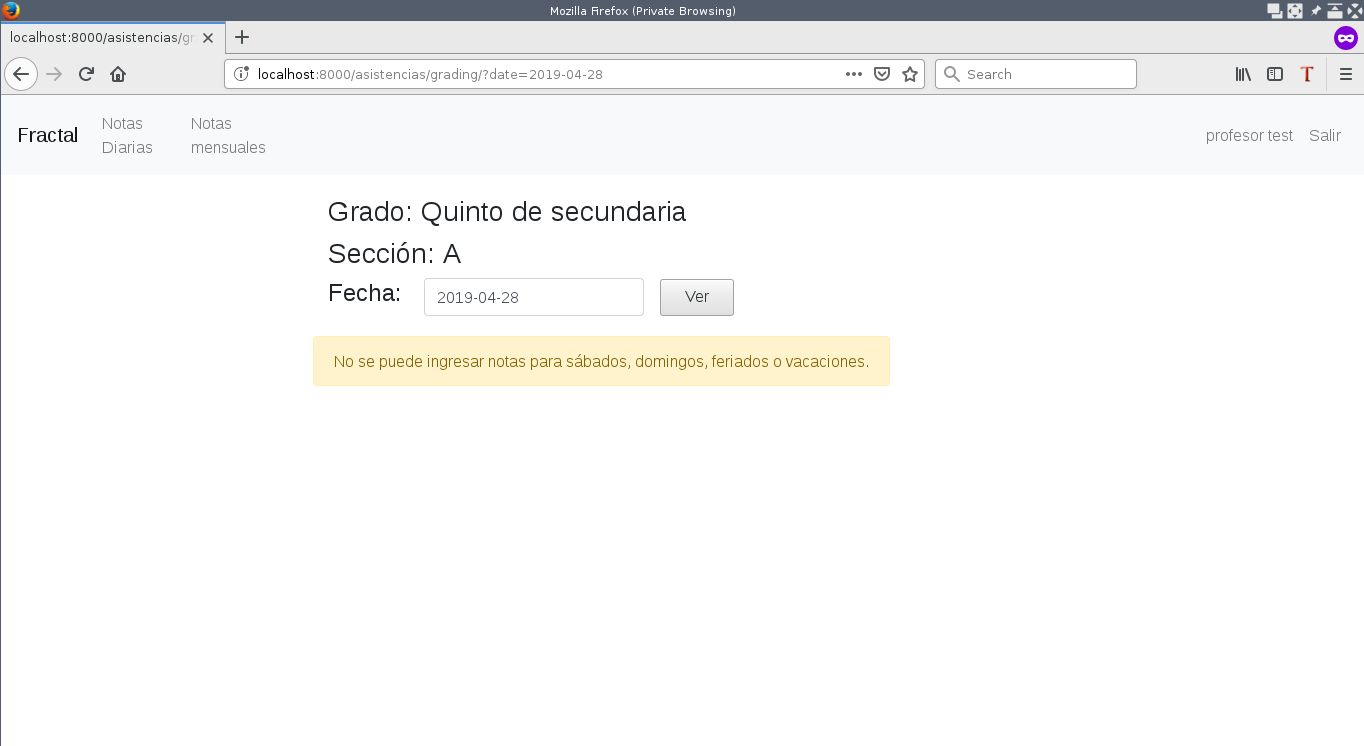
\includegraphics[width=0.8\textwidth]{images/profesor3.png}
  \caption{Registro en fecha no v\'alida}
  \label{fig:profesor3}
\end{figure}

Las notas se pueden ir llenando parcialmente. Por ejemplo, se puede llenar las notas de algunos
estudiantes, guardar el avance, y posteriormente continuar el llenado. El sistema mostrar\'a
todas las notas que fueron guardadas para esa fecha. Los estudiantes sin notas tendr\'an un gui\'on
``-'' en su lugar. Notar que 0 es diferente de ``-'',un cero se considera en el promedio del estudiante,
mientras que un gui\'on no.

\newpage
\section{Notas Mensuales}
La secci\'on de notas mensuales es similar a la secci\'on anterior. Esta vez, en lugar de ver la fecha,
se ve el periodo respectivo, como se aprecia en la figura~\ref{fig:profesor4}. De la misma forma se ve
la lista de todos los cursos.
\begin{figure}[ht]
  \centering
  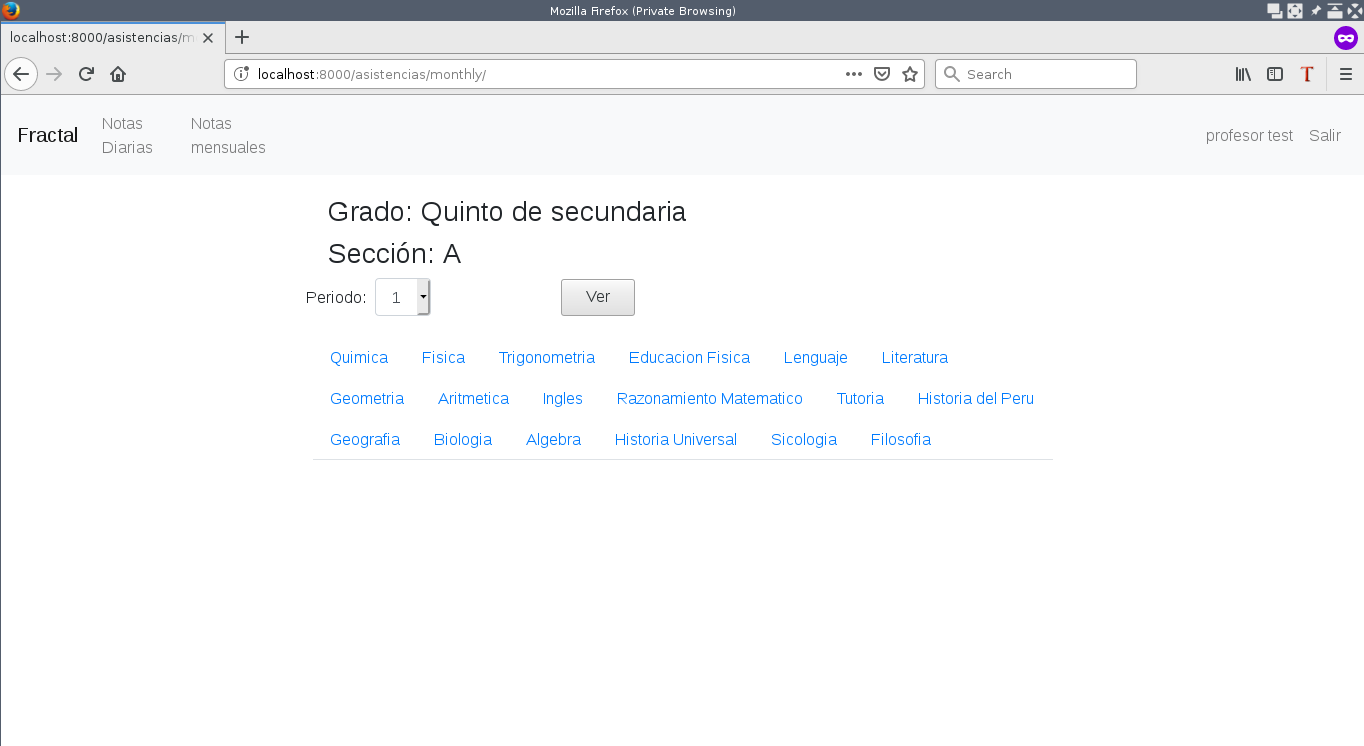
\includegraphics[width=0.8\textwidth]{images/profesor4.png}
  \caption{Registro mensual de notas}
  \label{fig:profesor4}
\end{figure}

Si se desea ingresar las notas para otro periodo, seleccionarlo en la lista y hacer click en ver.
De la misma forma que en la secci\'on anterior, las notas se pueden ir llenando parcialmente y el
bot\'on guardar solo guardar\'a las notas del curso que se muestra en pantalla.
\begin{figure}[th]
  \centering
  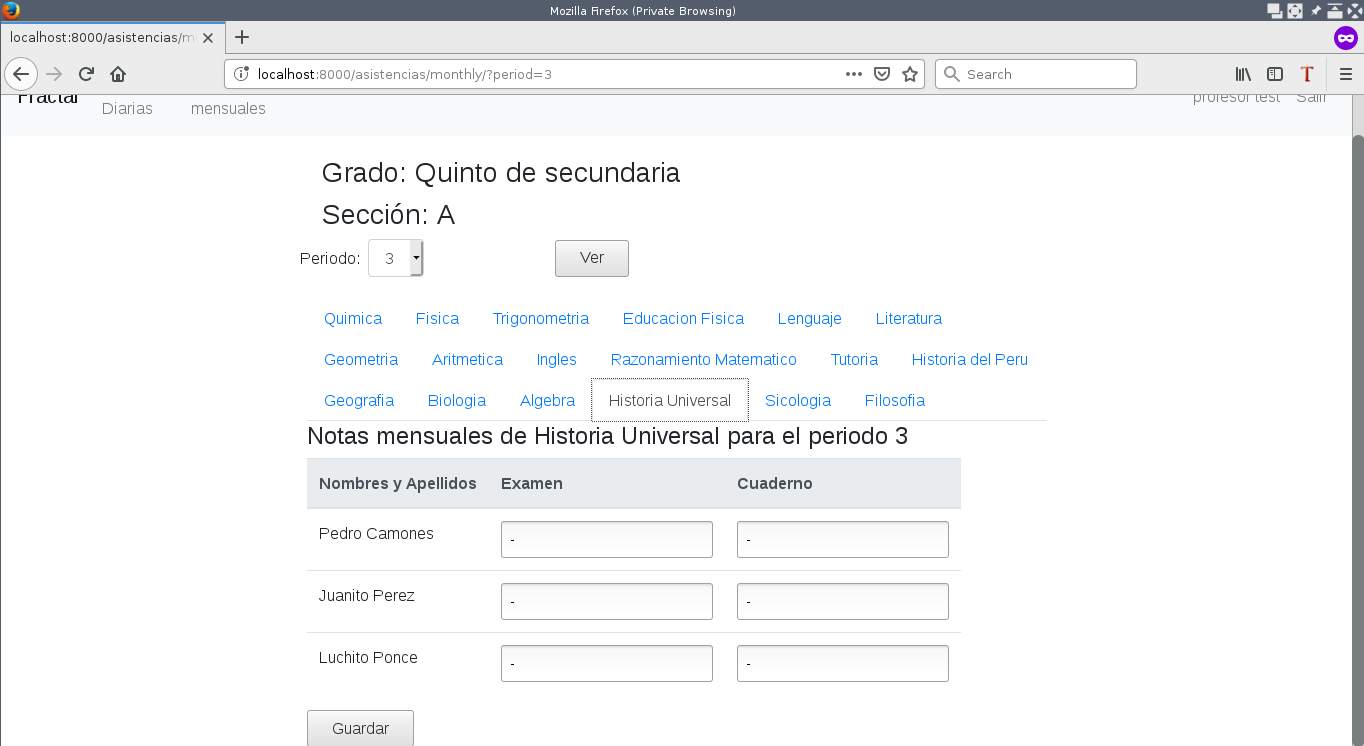
\includegraphics[width=0.8\textwidth]{images/profesor5.png}
  \caption{Registro mensual de notas}
  \label{fig:profesor5}
\end{figure}

Al salir del sistema no olvidar de hacer click en el bot\'on de la barra de navegaci\'on ``Salir''.
Cerrar la ventana no basta para cerrar la sesi\'on.
\end{document}

